% !TEX root = thesis.tex
\section{Resources}
\label{sec:resources}

It makes sense at this point (if not earlier), to discuss what language resources are. There are two main types of resources: corpora and tools which act on corpora. They are inextricably linked, but the approaches towards building, archiving, and using either differ. In this section, I will answer these questions: What resources are needed to take a language from no resources, to a thriving language with a large digital presence? And what resources are there?

For digital vitalisation, \citet{kornai2015new} proposes working on a pyramid approach: first build a corpus with active and engaged speakers, then l10n and i18n support; then word-level tooling such as spell checkers and morphological analysers; phrase and sentence level tooling such as parsers; and finally speech and character recognition and machine translation. This, in general, follows how most language development progresses. However, a finer-grained understanding of the tools would be illuminating.

\subsection{Types of language resources}

While an exposition of all possible natural language processing tools is beyond the scope of this thesis, it is worth going into some depth about some of them.

\subsubsection{Corpora}

All language resources ultimately depend upon corpora; without data, an algorithm does nothing. And yet not all corpora is the same, either. Data which has been cleaned - often using intensive manual effort and specific tooling - is far more efficient than generic buckets of sound clippings or text, although there are uses for both. Annotated corpora is more useful for specific tools, such as syntactic parsers or for morphological analysers. The type of annotation matters; for instance, interlinear glossed text (IGT) is an industry standard for displaying corpora in academic linguistics by displaying the original datum, a morphosyntactic gloss, and a translation. This is particularly useful for developers of morphological analysers and parsers, who are keen to interpret typological features of a language into their system.

Historically, the majority of corpora has been written corpora, due to the difficulty gathering, cleaning, and sorting large amounts of audio or video files. With the rapid escalation of computing power (mirrored and predicted by Moore's law \citep{schaller1997moore}, which observes that circuit board complexity doubles roughly every two years), and with the advent of large social media sites that allow users to upload their own language data (such as YouTube\footnote{\href{https://www.youtube.com/}{https://www.youtube.com/}. \last{May~2}}), audio and visual corpora are becoming more and more prevalent. Both types of corpora are relevant for LRLs; the former is useful for setting up fonts and characters and implementing them in Unicode, for spell checkers, and so on; while the latter can also be used to begin extracting phonemes \citep{kempton2014discovering, muller2017improving}, or for speech-to-text systems \citep{fraga2015active, fraga2015improving}, among other uses \citep{adams2017automatic}. Indeed, the proceedings of the workshop on Spoken Language Technologies for Under-resourced languages (SLTU), now in its sixth incarnation, show that using audio corpora to bootstrap language models is an active topic.\footnote{\href{http://www.mica.edu.vn/sltu2018/}{http://www.mica.edu.vn/sltu2018/}. \last{May~2}} The possibility of automatically extracting linguistic information from audio recordings has enabled field linguists to focus on recording data now, as well, instead of laboriously spending years transcribing a single language \citep{bird2014aikuma}.

There are other types of corpora. For instance, a bilingual or multilingual corpus is increasingly useful for NLP work on LRLs. By comparing aligned or identical translated texts from a source language, one can deduct systemic knowledge of the target language. When this is combined with typological features, one can swiftly build not just machine translators \citep{lewis2010haitian} but also grammars \citep{bender2016linguistic}. Even basic word lists can be useful in some instances; for instance, the Swadesh list of forty-odd words which are shown to be less likely to change over time \citep{swadesh1955towards} has been incredibly useful for showing language relationships and diachronic change. Another type of corpus would be photos of hand-written material or of particular font faces, for use in optical character recognition, where a knowledge of the alphabet or written resources can be used to develop digitised corpora. On a deeper level, wordnets (which track semantic relationships between various words), thesauri, and other semantically-enriched corpora can also be useful for research and language development.

Depending on the level of annotation and tooling done on a corpus, it often makes sense to include the code which cleaned the corpus in some way with the corpus itself. Using the data may require using a certain program. For instance, \citet{kempton2009finding} describe an automatic allophone induction tool using the TIMIT corpus \citep{garofolo1993darpa}, and they go into some depth discussing the tools needed to parse the well-known corpus, such as the SIL Phonology Assistant,\footnote{\href{https://software.sil.org/phonologyassistant/}{https://software.sil.org/phonologyassistant/}. \last{May~2} (Also an open source project on GitHub, at \href{https://github.com/sillsdev/phonology-assistant}{https://github.com/sillsdev/phonology-assistant}. \last{May~2}), although it wasn't open source when originally reviewed in 2008 \citep{dingemanse2008review}} or the SRILM extensible language modelling toolkit \citep{stolcke2002srilm}. However, unless the code is in some way bundled or its development is well-funded, a paper's combined tooling or workflow often isn't available explicitly.

\subsubsection{Code}
\label{sec:resources-code}

Before getting into the specifics of why code is decoupled from data, and what availability means (for that, see Section~\ref{sec:lrl-code}), it is worth exploring what types of computational resources are common for natural language processing (NLP) work. Here are some examples:

\begin{itemize}
  \item \textbf{ Font codecs}. Where a language has a new alphabet or characters which are not included in a standard alphabet, some of the first resources developed for that language are fonts and type-setting for the script. Often, languages may have a rich literary history but no digitisation of their native script; this was the case for Naskapi, and \citet{jancewicz2002applied,jancewicz2012cree} describe the process of setting up Naskapi Syllabics first for typewriters and later for computers over the past thirty years. This is explored further in Section~\ref{sec:naskapi}.
  \item \textbf{Language recognition}. An Cr\'ubad\'an \citep{scannell2007crubadan} uses trigram analysis to determine language identification for texts crawled from the internet; this means breaking down known wordlists into statistical frequency lists, by selecting three-character strings from a training set and seeing how well they match up on a target corpus. There are other types of language recognition software, using word frequencies, bigram analysis (especially for spoken data), and character recognition, for example.
  \item \textbf{Morphological parsers}. These are used to split words into their component pieces (morphemes).
  \item \textbf{Spell-checkers}. At their simplest, these perform string recognition on a dictionary of known forms. This works particularly well for isolating languages like Hawai'ian, where there is a surfeit of morphological differences for individual words. However, for agglutinative or slot-based languages, this requires a good deal more code under the hood, as the system needs to predict validity for morphemes within a word - both derivational (combinations occurring through historical processes, and often no longer productive for grammatical new forms) and inflectional (productive word-building demanded by morphosyntactic processes).
  \item \textbf{Tokenizers}\footnote{Editorial note: While this thesis generally follows British or Canadian spelling rules, for certain terms the American system is used to conform to popular keywords in the scientific literature.} are used to split strings into tokens. Most often, this involves simply splitting words out of a sentence - to a computer, the space character is no different than an alphanumeric one, and so splitting on the character is important for other code to know where a word ends and begins.
  \item \textbf{Lemmatizers} group together inflected forms under one heading, so that a word with many variants can be identified as the having the same lemma, or root.
  \item \textbf{Part-of-speech (POS) taggers} figure out the syntactic function of a particular word within a given context, and are useful for parsers and for word-sense disambiguation. These are most often rule-based, and involve a knowledge of the language's syntactic functions, as well as depending upon morphological parsing for variant forms.
  \item \textbf{Named Entity Recognition (NER)} involves extracting proper names from a text - for instance, any persons, businesses, times, currencies, and so on. This is particularly useful for parsing large corpora to quickly find relevant features; for instance, extracting a politician's name from years of newspaper corpora is a common task for NLP researchers.
  \item \textbf{Syntactic parsers} are used to understand the syntactic function of words within a sentence or phrase, and are particularly useful for machine translation. However, knowing the syntax is also useful for other tools such as sentiment analysis or NER, as it provides a finer-grained understanding of the text and context.
  \item \textbf{Speech-To-Text (STT)} and \textbf{Text-To-Speech (TTS)} are systems which, understandably, convert written corpora into audio, and vice versa. Generally these involve a fair amount of work and a large corpora, although there are systems which are able to produce reasonably useful systems from scarce data (see discussion above). This is useful for a variety of uses, from automatic transcription to robot voice systems to geographical map guidance.
  \item \textbf{Machine Translation (MT)} systems automatically transfer information encoded in one language into another, and generally involve statistical knowledge of the source and target language and complicated grammars which are either encoded directly or built on universal translation systems. The arguably most common MT system today, Google Translate, originally used statistical machine translation with multilingual aligned texts, but is now switching to a neural network system, using more complicated machine learning algorithms \citep{google2016google}.
\end{itemize}

There are more tools which could be named here. The key point to take away is that language development is neither an easy task involving a weekend's work by a team of volunteers, nor a matter of developing a finite set of tools. Instead, it is a gradated process that involves consistent development and fine-tuning, generally involving dozens if not hundreds of language developers working on various parts of the process. One difficulty in this process is finding out what has been done before, to avoid duplicated work. It is to solve this need that resource aggregators exist.

\subsection{Resource aggregators}
\label{subsec:resource-aggregators}

I have already mentioned that An Cr\'ubad\'an \citep{scannell2007crubadan} is a good location to find monolingual texts from the web; however, this is but one of many corpora that might be of use to linguists, language activists, and to NLP practitioners. To find other resources can be an overwhelming task. \citet{unesco11directory} for instance itemises hundreds of such resources. To help solve this issue, there are a non-trivial number of large organisations and databases where it is possible to find resources - dictionaries, academic references, and occasionally software - on low resource languages. To give more of an idea of what these resources are like, here are some major examples:

\begin{itemize}
\item The Unicode Common Local Data Repository (CLDR) "provides key \\ building blocks for software to support the world's languages, with the largest and most extensive standard repository of locale data available."\footnote{\href{http://cldr.unicode.org/}{http://cldr.unicode.org/}. \last{May~2}} There are dozens of scripts available in Unicode.\footnote{\href{https://www.unicode.org/standard/supported.html}{https://www.unicode.org/standard/supported.html}. \last{May~2}}

\item The Endangered Languages Project (ELP), described above and in \citet{lee2016assessing} and online\footnote{\href{http://www.endangeredlanguages.com/}{http://www.endangeredlanguages.com/}. \last{May~2}} has information on many under resourced languages.

\item Ethnologue, which is both a book \citep{lewis2009ethnologue} and an online resource,\footnote{\href{https://www.ethnologue.com/}{https://www.ethnologue.com/}. \last{May~2}} is the most comprehensive resource describing the world's languages, such as population size and the general geographic locations of speakers. It is published by SIL International, an evangelical Christian non-profit organisation, and has proprietary paywalls for repeated access to content. Many SIL entries for specific languages include academic references.

\item Glottolog\footnote{\href{http://glottolog.org/}{http://glottolog.org/}. \last{May~2}} is an open source alternative to Ethnologue, developed at the Max Planck Institute for Evolutionary Anthropology. It has over 180,000 references, with information on over eight thousand languages.\footnote{The astute reader will note that this is more than the amount of languages mentioned in \citet{lewis2009ethnologue}. The definition of what constitutes a language differs, and so the numbers can fluctuate between sources.} \citep{hammarstrom2015glottolog}

\item Omniglot, "the online encyclopaedia of writing systems and languages",\footnote{\href{http://omniglot.com}{http://omniglot.com}. \last{May~2}} contains information on writing systems for around a thousand languages. \citep{ager2008omniglot}

\item The Online Database of Interlinear Text (ODIN)\footnote{\href{http://odin.linguistlist.org}{http://odin.linguistlist.org}. \last{May~2}} is a multilingual repository of annotated language data for 1274 languages.\footnote{Noted as of January 13, 2010 at \href{http://odin.linguistlist.org}{http://odin.linguistlist.org}. \last{May~2}} The database is formed by crawling scholarly articles on the web and looking for IGT examples. As well, "ODIN was developed as part of the greater effort within the GOLD Community of Practice \citep{farrar2007gold} and the Electronic Metastructure for Endangered Languages Data efforts (EMELD),\footnote{\href{http://emeld.org/}{http://emeld.org/} (\last{May~2}) and \citet{farrar2002common}} whose goals are to promote best practice standards and software, specifically those that facilitate interoperation over disparate sets of linguistic data." \citep{lewis2010developing}

\item The Open Language Archives Community (OLAC) is a worldwide virtual library of language resources \citep{simons2003open},\footnote{\href{http://www.language-archives.org/}{http://www.language-archives.org/}. \last{May~2}} and contains thousands of cross-references to resources both on the web and in print form.

\item Wikipedia,\footnote{\href{https://www.wikipedia.org/}{https://www.wikipedia.org/}. \last{May~2}} "the largest and most popular general reference work on the Internet" \citep{wiki:Wikipedia} has a nontrivial amount of articles on low-resource languages, many of which have references themselves to scholarly work. \citet{kornai2013digital}, among others, notes that Wiki\-pedia is one of the first ports-of-call for new language communities, and while it is not a precondition for having corpora on the web, it is a {\it sine qua non} for digital vitalisation. Thus Wikipedia has two purposes; documenting the language and its community (for instance, in the Naskapi Language article\footnote{\href{https://en.wikipedia.org/wiki/Naskapi\_language}{https://en.wikipedia.org/wiki/Naskapi\_language}. \last{May~2}}), and providing a space for corpus development in the target language itself (for instance, as in the Gaelic wikipedia\footnote{\href{https://gd.wikipedia.org/wiki/G\%C3\%A0idhlig}{https://gd.wikipedia.org/wiki/G\`aidhlig}. \last{May~3}}).

\item The World Atlas of Language Structures (WALS) \citep{wals} is a directory of typological features which also includes academic references for many of the over two thousand languages presented. WALS is a curated resource, largely made by a team of 55 experts, and hosted by the Max Planck Institute for Evolutionary Anthropology (the same as Glottlog, and as other resources such as PHOIBLE\footnote{\href{http://phoible.org/}{http://phoible.org/}. \last{May~2}} \citep{phoible} and DOBES\footnote{\href{http://dobes.mpi.nl/}{http://dobes.mpi.nl/}. \last{May~2}} \citep{wittenburg2003dobes} related to taking an inventory of language structures).
\end{itemize}

There are other resources: the CLARIN Virtual Language Observatory,\footnote{\href{https://vlo.clarin.eu}{https://vlo.clarin.eu}. \last{May~2}} the Linguistic Data Consortium at UPenn,\footnote{\href{https://www.ldc.upenn.edu/}{https://www.ldc.upenn.edu/}. \last{May~2}} the ELRA,\footnote{\href{http://catalog.elra.info/en-us/}{http://catalog.elra.info/en-us/}. \last{May~2}} META-SHARE,\footnote{\href{http://www.meta-share.org/}{http://www.meta-share.org/}. \last{May~2}} the Association for Computational Linguistics' Wiki,\footnote{\href{https://aclweb.org/aclwiki/Main_Page}{https://aclweb.org/aclwiki/Main_Page}. \last{May~2}} the NICT Universal Catalogue,\footnote{\href{https://www.nict.go.jp/index.html}{https://www.nict.go.jp/index.html}. \last{May~2}} LT World\footnote{\href{http://www.lt-world.org/}{http://www.lt-world.org/}. \last{May~2}} and so on. Providing an exhausting list would be an impossible task, as there are often collections for each specific language family or region. For instance, Afranaph\footnote{\href{http://www.africananaphora.rutgers.edu/home-mainmenu-1}{http://www.africananaphora.rutgers.edu/home-mainmenu-1}. \last{May~3}} is a database of research on African languages. More pertinently, now that it is clear what resources are, and that it is possible to at least get a basic idea of what resources there are for a given language, what resources are relevant to low resource languages?

\subsection{BLARK and LRE maps}
\label{subsec:blark-and-lre-maps}

\citet{soria2017digital} briefly mention `digital language survival kits' as one of the motivations for their paper - these are explicated more fully on the Digital Language Diversity Project's site.\footnote{\href{http://www.dldp.eu/en/content/digital-language-survival-kit}{http://www.dldp.eu/en/content/digital-language-survival-kit}. \last{May~2}} This project is an EU initiative, through the Erasmus+ programme, and it aims to identify needs and provide `kits' for certain European low resource languages - specifically Basque, Breton, Karelian and Sardinian.

The use of the word `kit' is informative, as there is  pre\"{e}xisting literature on this topic regarding the BLARK, or Basic Language Resource Kit. BLARK was developed by a joint initiative between the European Network of Excellence in Language and Speech (ELSNET), a European international umbrella for 145 different organisations in 29 countries, and the European Language Resources Association (ELRA), and first outlined in \citet{krauwer1998elsnet}. The BLARK is defined as the "minimal set of language reosources that is necessary to do any precompetitive research and education at all." \citep[4]{krauwer2003basic} In general, this comprises "written language corpora, spoken language corpora, mono- and bilingual dictionaries, terminology collections, grammars, modules (e.g. taggers, morphological analysers, parsers, speech recognisers, text-to-speech), annotation standards and tools, corpus exploration and exploitation tools, bilingual corpora, etc."

\citet{krauwer2003basic} has a comprehensive matrix in the appendix outlining technology that would be needed to provide a BLARK for Dutch, as outlined in a workshop documented in \citet{binnenpoorte2002towards}. In another paper, \citet{maegaard2006blark} under NEMLAR (Network  for  Euro-Mediterranean  LAnguage  Resources) outlined the specific language resource needs for Arabic in a BLARK table, noting the importance of certain modules for better language coverage. Both of the BLARK grids for Arabic provided in that paper are included here, in Figures~\ref{fig:blark1} and \ref{fig:blark2}, as they very usefully show not only the state of HLT resources for Arabic at the time, but also the categories thought sufficient. They also point out how both written and spoken language tools need to be developed, and can't be considered in isolation. Their categories - `prosody prediction', `alignment', `shallow parsing', and so on - are all terms which refer to a suite of resources that each reflect hundreds of papers from within the computational linguistics community, which Section~\ref{sec:resources-code} briefly explicated.

\begin{figure}
 \centering
 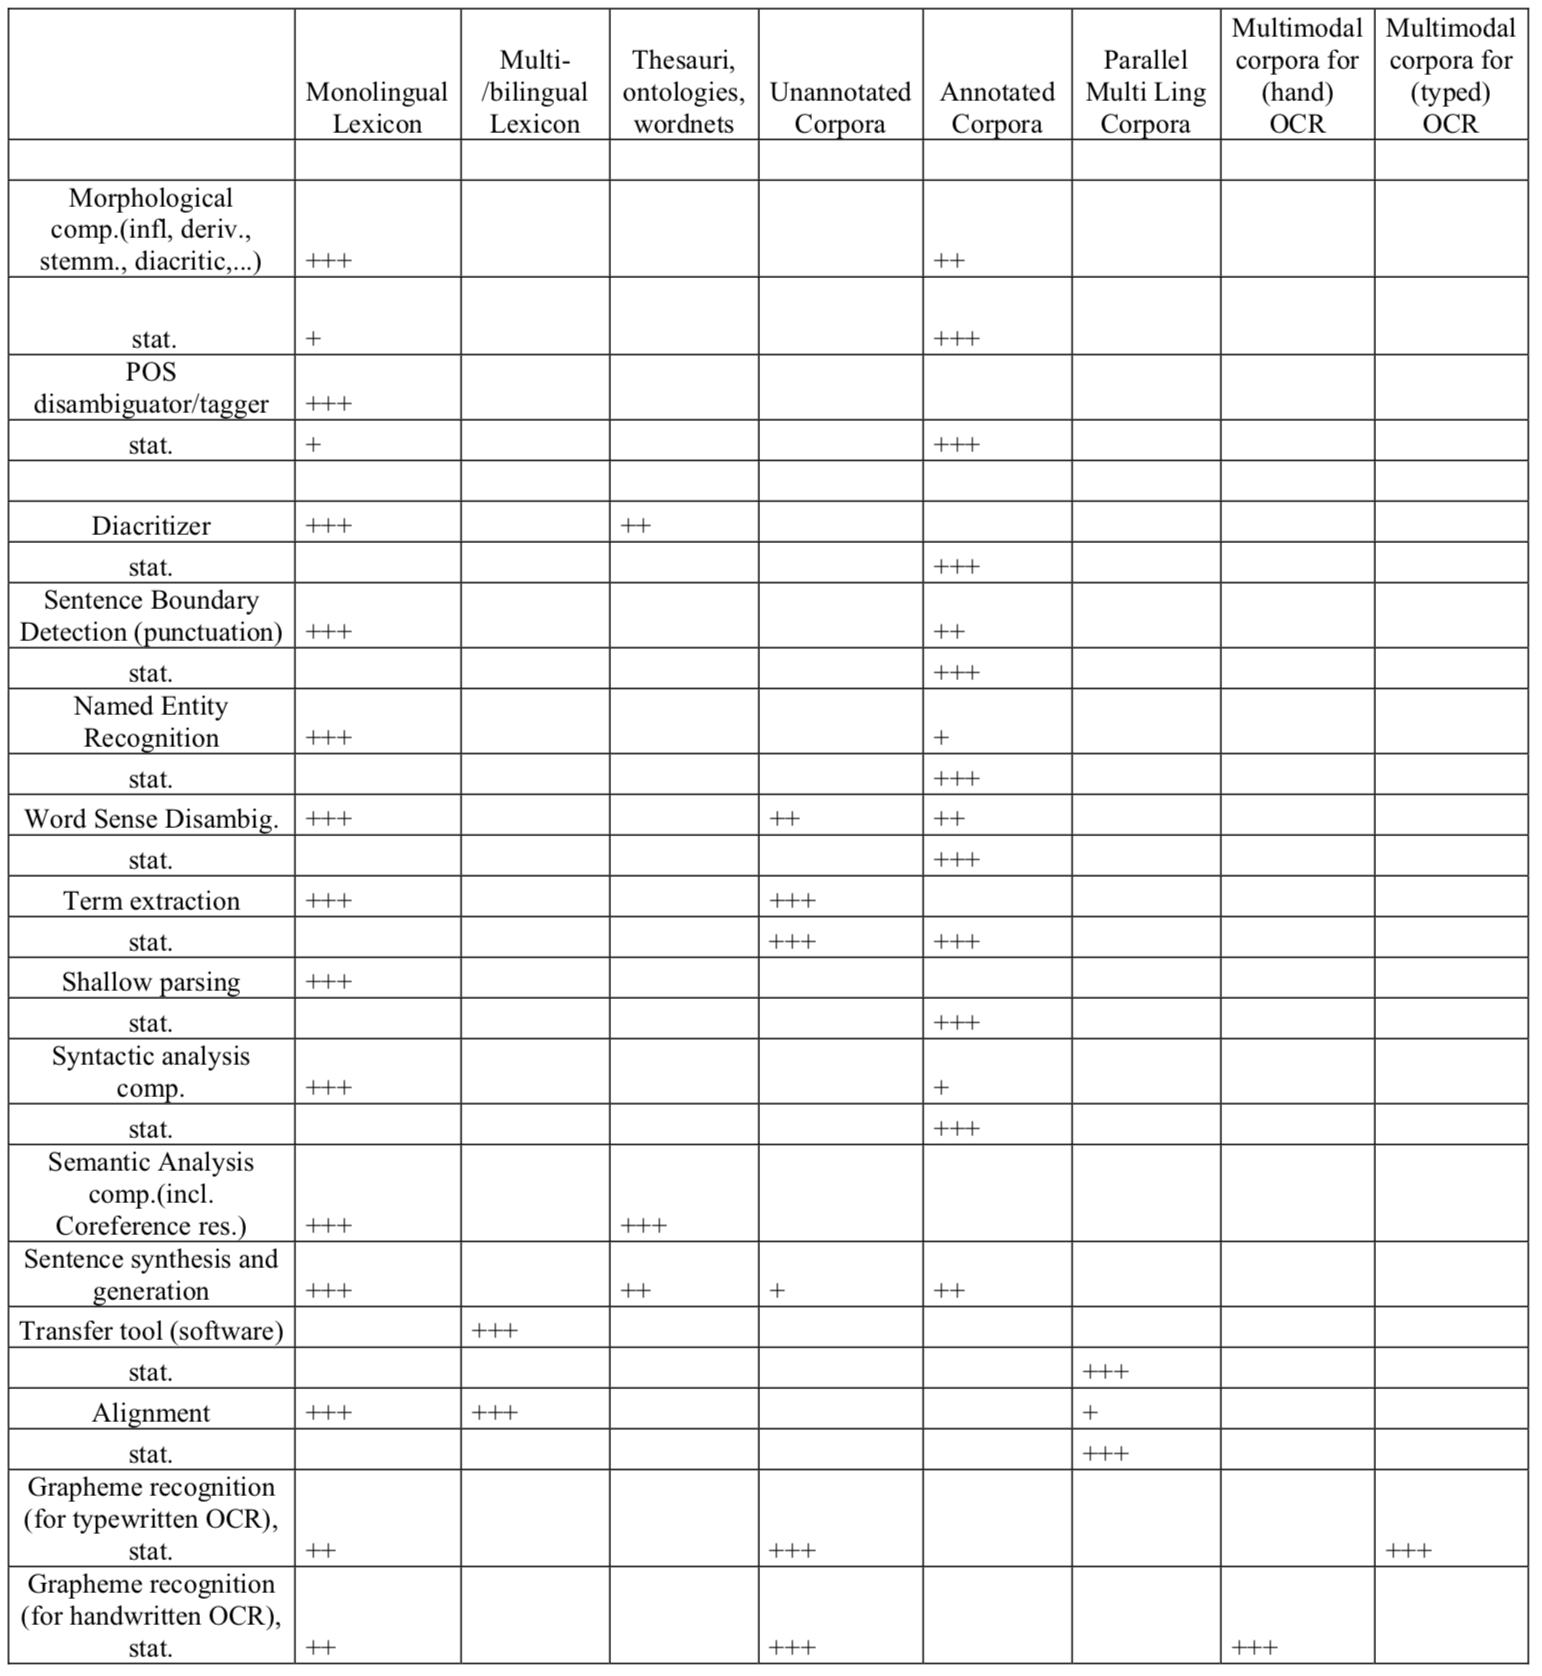
\includegraphics[width=1\textwidth]{img/blark1.png}
 \caption{A BLARK graph for Arabic, with written language applications and corresponding HLT modules, marked with importance \citep[775]{maegaard2006blark}}
 \label{fig:blark1}
\end{figure}

\begin{figure}
 \centering
 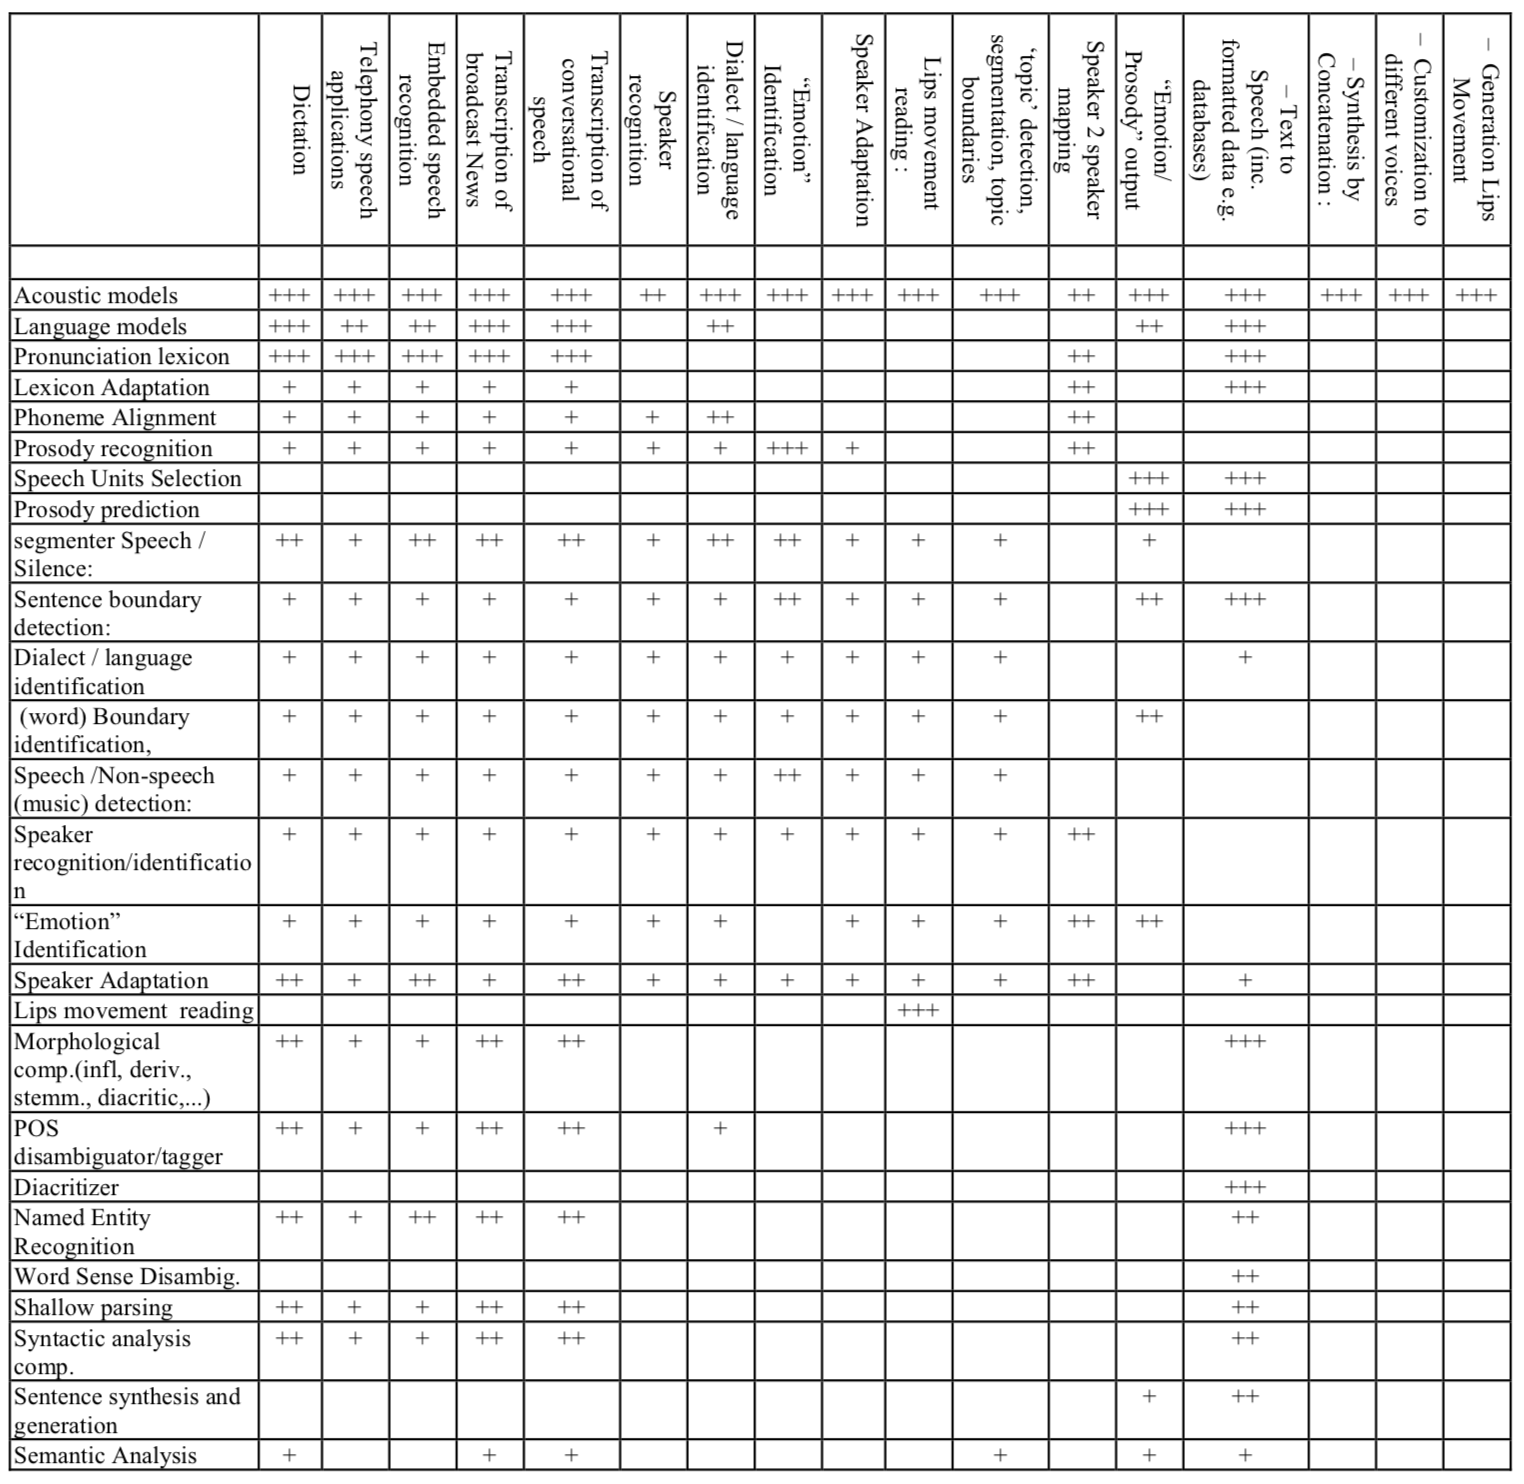
\includegraphics[width=1\textwidth]{img/blark2.png}
 \caption{A BLARK graph for Arabic, with speech language applications and corresponding HLT modules, marked with importance \citep[776]{maegaard2006blark}}
 \label{fig:blark2}
\end{figure}

The BLARK process - auditing a language, using a grid to identify what corpus and resource needs are necessary for language resources - has now been applied to Swedish \citep{elenius2008language} and Bulgarian \citep{simov2004language}, and numerous South African languages \citep{grover2011south}, among others.

Unfortunately, BLARK (or ELARK, purportedly a more sophisticated version of BLARK for industry described in \citet{mapelli2003report}, according to \citep{grover2011south}) is a large grid, and may not work for languages without extensive funding models or support. For this, there is a smaller BLARK version, the BLARKette, which should work for low resource languages (although how a smaller version of a minimal set could be provided usefully is not clear).

\begin{quote}
In order to accommodate this problem we have proposed the definition of a scaled down, entry-level version of the BLARK, targeting exclusively the research and (especially) the education community. It should be light and compact, not too demanding in terms of hard and software requirements, cheap, free from IPR issues, and ideally small enough to fit on a CD or DVD. We expect to release a first document, with tentative summary specifications, towards the end of 2006. Check the ELSNET site for news. \citep{krauwer2006strengthening}
\end{quote}

The model of transportation for this - a CD, instead of a downloadable resource - shows that the concept has not aged well. There is also a surfeit of references of BLARK or BLARKette in the past decade in the literature - \citet{krauwer1998elsnet} only has 31 references on Google Scholar (an imperfect but effective metric).\footnote{\href{https://scholar.google.com/scholar?cites=5069727220703395724}{https://scholar.google.com/scholar?cites=5069727220703395724}. \last{May~2}} What happened? It is most likely (in my opinion) that building a BLARK for a language is too complex for language groups to perform, and lacks proper incentives. It requires an authoritative and intimate knowledge of a language's space by many researchers, all of whom must come together to identify gaps, often from proprietary institutions. This is a difficult task.

But this effort, in some sense, has expanded into LRE (Language Resources and Evaluation) maps within Europe. As described in \citet{calzolari2010lrec, del2014lremap, mariani2015language, del2015visualising}, the Language Resources and Computation (LREC) conference organisers began asking conference participants who had submitted papers to fill out basic language resource grids when submitting papers. This effort was extended to ten different computational linguistics conferences, covering most large European languages and four regional Spanish languages. This data has been collected into matrices and a database that reflects language resources for a variety of languages. To date, this is the most comprehensive review of NLP per language that I am aware of, with 4395 entries - however, it is worth noting that it is limited in scope. The 133 less-common languages represented in the LRE map represent only 414 entries. An example of the matrix for the high resource languages can be seen in Figure~\ref{fig:lre}, which is a map of resources for various languages, cut off with a lower bound of 50 citations per resource type.

\begin{figure}
 \centering
 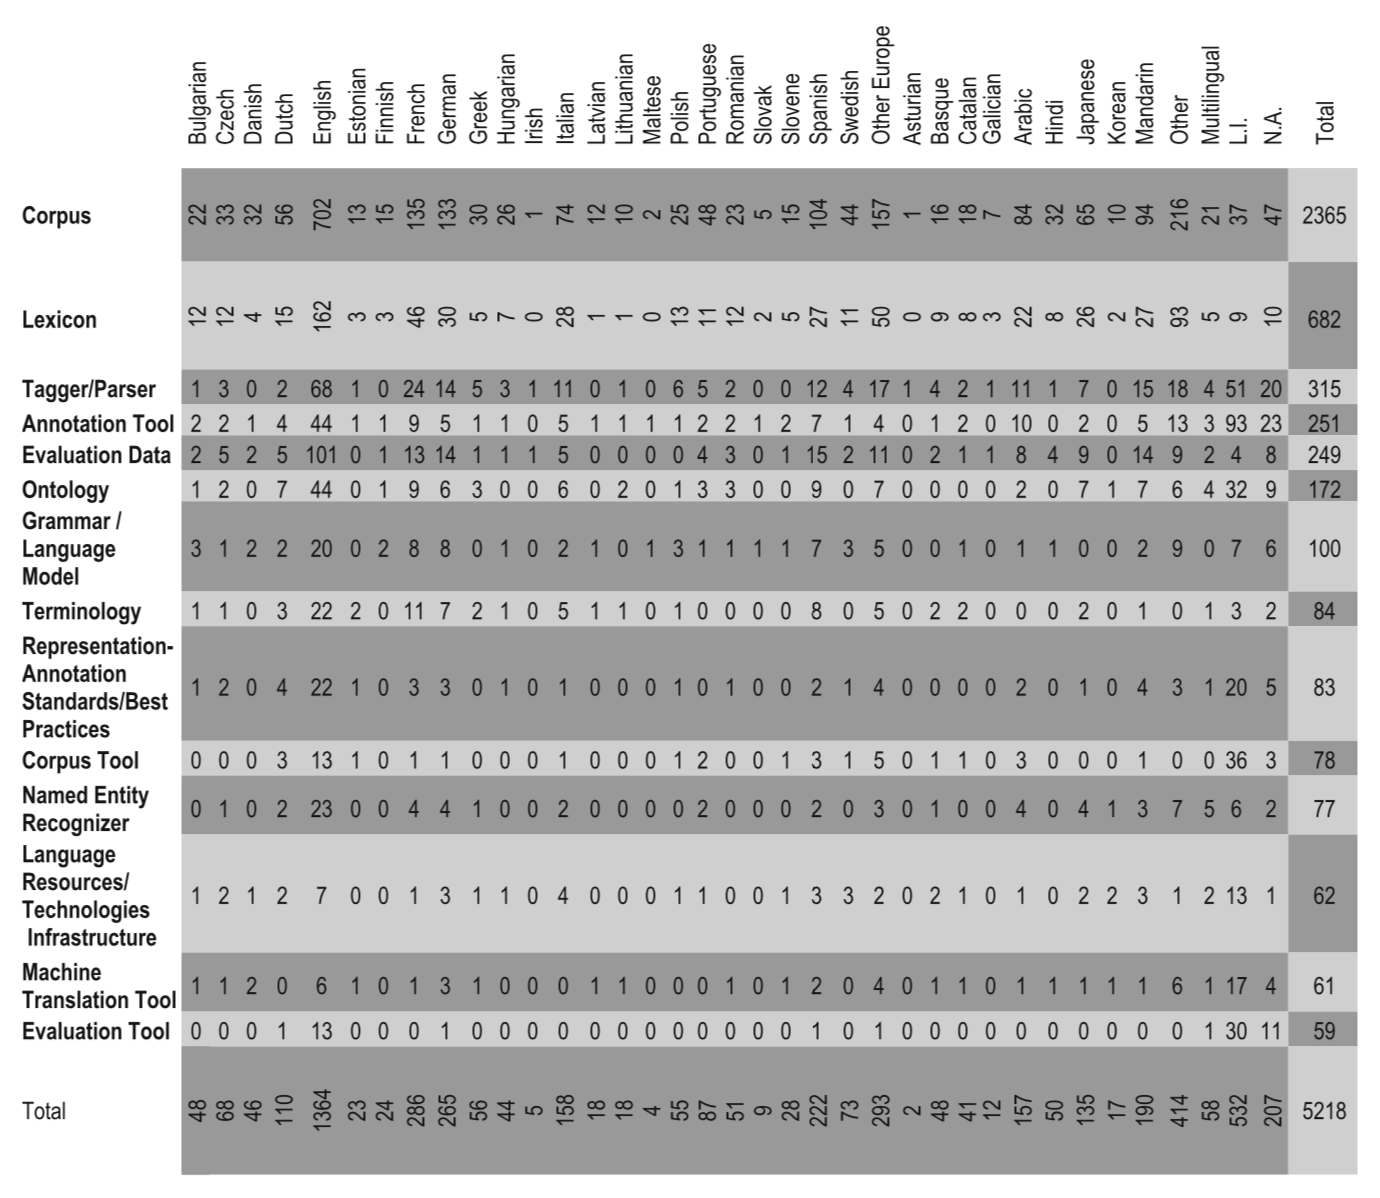
\includegraphics[width=1\textwidth]{img/lre.png}
 \caption{LRE maps for high resource languages \citep[460]{mariani2015language}}
 \label{fig:lre}
\end{figure}

Several authors working on LRE maps are also authors of the \citet{soria2017digital} paper; extending the LRE maps for low resource languages, and then intensifying efforts to develop low-hanging fruit for low resource languages is a logical next step for this research. The focus on European languages is expected; this may stem from the fact that LREC, the main conference series from which LRE data was drawn, is run by the European Language Research Association (ELRA). This fragmentation of the field is unsurprising, and happens in the reverse, as well: for example, \citet{paricio2010new} cites a framework for upgrading low resource languages which is explained in a research paper written in Spanish, and, anecdotally, around half of the papers presented at the Ryukyuan Heritage Language Society's conference in Tokyo in 2012 (which I attended) were presented in Japanese. This is not to say that fragmentation and diversity of linguistics in academia is something to be avoided, but rather that it is a hurdle to be noted and worked with to avoid repeated work and splintered efforts.

% Note: Made redundant by other examples in the text. I don't think this is needed.
%\subsection{The current state of language diversity}
%In this section, I am going to briefly go into detail about what diversity means for linguistics. This will be useful later for explaining how related languages can be used to bootstrap work in similar languages. For instance, Irish spell-checkers and constitutional corpora from the EU can be used by Scottish Gaelic speakers with some tweaks in order to further improve their own systems.

\subsection{Who makes resources for languages?}
\label{subsec:who-makes-resources}

Different groups  work on different stages of language development, and each brings their own perspective, intentions, tools, and achievements. Abstractly, the groups could most easily be separated into language communities and linguists, and the fields of computational linguistics and NLP. The first group are those - often not computational linguists by training or NLP researchers - who want their own language or the language they are studying to exist digitally in some form. The initial step is generally to adopt any language script, whether  pre\"{e}xisting or ready-made for the language by linguists (for examples of this, see the Endangered Alphabets Project\footnote{\href{http://www.endangeredalphabets.com/}{http://www.endangeredalphabets.com/}. \last{May~2}}) into Unicode, a standard for consistent character representation.\footnote{\href{https://unicode.org/}{https://unicode.org/}. \last{May~2}} There are linguistic research groups that focus on this problem; for instance, the Script Encoding Initiative at Berkeley.\footnote{\href{http://linguistics.berkeley.edu/sei/index.html}{http://linguistics.berkeley.edu/sei/index.html}. \last{May~2}}

Some of the people involved in this process may be computational linguists. \citet{bender2016linguistic} makes a distinction between the fields of computational linguistics and NLP: "computational linguistics is used to describe research interested in answering linguistic questions using computational methodology, while natural language processing describes research on automatic processing of human language for practical applications." It should be clear here that computational linguistics is a subfield of linguistics, and that the two are not always in sync, as for instance \citet{kay1997proper} points out when discussing improving MT processes by using informed linguists to build semi-supervised systems. \citet{bender2010grand, bender2016linguistic} go further, suggesting that understanding language typology can drastically help with multilingual NLP.

Meanwhile, many experts in NLP would not consider themselves computational linguists, but developers, just as many language developers would not consider themselves linguists. While navigating the field or looking at resources, it is important to keep these distinctions in mind, as they inform narratives concerning resource generation, scope, and efforts.

Another hurdle which was briefly alluded to earlier was the plethora of large organisations, databases, or projects dedicated to cataloguing low resource languages. Each of these has differences in scope, funding, and incentives. However, large organisations are not the only groups working on language development, digital ascent, language revitalisation, or any other shared focus that relates to low resource languages.

As \citet{hammarstrom2015unesco} points out, "language documentation and description is an extremely decentralized activity, carried out by missionaries, anthropologists, travellers, naturalists, amateurs, colonial officials, ethnographers and not least linguists over several hundred years." Language communities, amateur and professional linguists, educators, and language policy setters are most often involved in standardising a language and helping to document and revitalise low resource languages. Digitally, amateur computational linguists and coders who are first-language speakers of their respective LRLs are often the first to work on translating or migrating resources; this group is also often the first to set up wikipedias in a local language (although this often leads to enthusiastic loners working outside of the main language communities \citep{soria2017digital}). These researchers don't necessarily work only on their own languages; for instance, the {\it Indigenous Languages and Technology} email listserv\footnote{\href{http://www.u.arizona.edu/~cashcash/ILAT.html}{http://www.u.arizona.edu/~cashcash/ILAT.html}. \last{May~3}} connects hundreds of different people interested in this area of research, without focusing on a single language.

Beyond these groups, universities and local governments can also often develop language resources for low resource languages, as was the case with \citet{rognvaldsson2009icelandic} and with First Voices, a Canadian First Nations archiving platform.\footnote{\href{https://fv.nuxeocloud.com/}{https://fv.nuxeocloud.com/}. \last{May~3}} Non-profits are also common in the language resource development space; examples include the Endangered Language Alliance,\footnote{\href{http://elalliance.org/}{http://elalliance.org/}. \last{May~3}} Terralingua,\footnote{\href{http://terralingua.org/}{http://terralingua.org/}. \last{May~3}} the Foundation for Endangered Languages,\footnote{\href{http://www.ogmios.org/index.php}{http://www.ogmios.org/index.php}. \last{May~3}}, the Living Tongues Institute for Endangered Languages,\footnote{\href{https://livingtongues.org/}{https://livingtongues.org/}. \last{May~3}} and so on.

After these groups, large grant-driven institutions such as CLARIN or the NSF fund a large portion of language development, along with industry giants such as Google or Xerox, and large military research arms such as DARPA. Sometimes grants come from philanthropic organisations, like the Bill and Melinda Gates foundation \citep{penfield2006technology}, or philanthropic arms of enterprises, such as Rosetta Stone's work on some indigenous North American languages.\footnote{\href{https://www.rosettastone.com/endangered/projects}{https://www.rosettastone.com/endangered/projects}. \last{May~3}}

Unfortunately, the lion's share of the overall funding for language development goes to languages which are already resourced.

\begin{quote}
Over the years the EU has invested massively in the development of language and speech technology, and many dedicated R\&D programmes have had a significant impact on its advancement, including applications oriented towards solving the multilinguality problem... Unfortunately the strong industrial bias of recent EU programmes has led to a situation where the major part of the funding for language and speech technology goes to the major languages. This is not surprising, as industrial players will prefer to invest in the development and deployment of technologies for larger markets. As a consequence there has been only marginal support for the development of language and speech technology for the language communities that do not constitute profitable markets. As the development cost of such technologies is independent of the number of speakers of a language ("all languages are equally difficult") this has created a very unbalanced situation. \citep{krauwer2006strengthening}
\end{quote}

Or:

\begin{quote}
Were it not for the special attention DARPA, one of the main sponsors of machine translation, devoted to Haitian Creole, it is dubious we would have any MT aimed at this language. There is no reason whatsoever to suppose the Haitian government would have, or even could have, sponsored a similar effort \citep{spice}. \citep[9]{kornai2013digital}
\end{quote}

The attentions of DARPA and IARPA (Intelligence Advanced Research Proj\-ects Activity, a US institution modelled after DARPA but focusing on national security and not military concerns) on low resource languages is clear, and these are only two branches of the US military-industrial complex. The Low Resource Languages for Emergent Incidents (LORELEI),\footnote{\href{https://www.darpa.mil/program/low-resource-languages-for-emergent-incidents}{https://www.darpa.mil/program/low-resource-languages-for-emergent-incidents}. \last{May~3}} Machine Translation for English Retrieval of Information in Any Language (MATERIAL)\footnote{\href{https://www.iarpa.gov/index.php/research-programs/material}{https://www.iarpa.gov/index.php/research-programs/material}. \last{May~3}} and Babel\footnote{\href{https://www.iarpa.gov/index.php/research-programs/babel}{https://www.iarpa.gov/index.php/research-programs/babel}. \last{May~3}} projects explicitly mention `low resource languages` as research areas. The budget for these projects is not public, but can be safely assumed to be in the tens of millions of dollars.\footnote{\href{https://www.popularmechanics.com/technology/security/a17451/iarpa-americas-secret-spy-lab/}{https://www.popularmechanics.com/technology/security/a17451/iarpa-americas-secret-spy-lab/}. \last{May~3}} As well, the general public can't know how these tools and projects are then utilised, and whether it is in the best interest of speakers of low resource languages. It is safe to assume that, unless the speakers are US citizens or allies, they are not, as the American military's stated goal is to ensure security for its own nationals. This means that any work done by these bodies, and by researchers connected to them, can be seen as controversial.

Another good example of where funding and incentives for language development can be controversial would be Ethnologue, which rate limits and has a paywall guarding usage of their database, even though they are widely recognised as one of the best informed databases for language data. This paywall can be triggered by viewing a non-trivial amount of pages (around five) for languages on the site. While this is philosophically no different than asking researchers to buy \citet{lewis2009ethnologue}, this data is the most widely used, and this paywall was only implemented in late 2015.\footnote{\href{https://www.ethnologue.com/ethnoblog/m-paul-lewis/ethnologue-launches-subscription-service\#.VmA0hspth0o}{https://www.ethnologue.com/ethnoblog/m-paul-lewis/ethnologue-launches-subscription-service\#.VmA0hspth0o}. \last{May~3}}

SIL International is also the standardising body in charge of the ISO 639-3 standard, which is the most widely used language code. By having a paywall on their data, they exclude the general public from having control of codes for their own languages. SIL has also come under criticism for their Christian missionary work, as it can be viewed as complicit in culture change, and by extrapolation, ethnocide \citep{dobrin2009sil, dobrin2009practical, everett2009don}. This is just one example - and most likely one of the most extreme, not counting military work on languages used by insurgents in wars (implied above) - of how organisations working on language resources may influence the work itself.

The funding of language resource development matters, because the way that the language community approaches language development affects the chance of survival for the language. This is one of the reasons that \citet{grenoble2016response} pointed out that `language vitality' is a more politically correct term to use than `language endangerment', as it takes the focus away from loss and focuses attention on language ascent. Another reason that language funding matters is because the major players with funding will generally be able to out manoeuvre smaller groups with different resources. This can enforce language shift, and can render resources created by individual developers moot. For instance, the secwepemc-facebook\footnote{\href{https://github.com/kscanne/secwepemc-facebook}{https://github.com/kscanne/secwepemc-facebook}. \last{May~2}} tool developed to automatically translate Facebook into low resource languages, created by the late Neskie Manuel for his native Secwepemcts\'in, is no longer an active project and has not been updated, rendering it obsolete with Facebook UI changes, while automatic translation is provided for high resource languages natively by Facebook. Scannell, who helped port the secwepemc-facebook tool to Greasemonkey\footnote{\href{https://www.greasespot.net/}{https://www.greasespot.net/}. \last{May~3}} for use on Mozilla Firefox\footnote{\href{https://www.mozilla.org/en-US/firefox/}{https://www.mozilla.org/en-US/firefox/}. \last{May~3}} was one of the authors of \citet{streiter2006implementing}, which suggested that developers for low resource languages use open source software pools in order to pool resources to enable them to overcome this - among other - issues facing low resource languages in particular.

As in Section~\ref{subsubsec:response}, covering all of the potential issues with funding and the politics of language development is well beyond the scope of this paper. However, focusing on how open source can help low resource languages is not. But first; what do I mean by `open source'?
